\chapter{Modelling claims}
\label{chap:claims}

Using \RA{} usually starts with either selecting an existing or creating a new parameterization. If you start \RA{} for the first time, there are already several models with illustrative parameterizations made available for an easy introduction to the software.\footnote{If you produce any teaching material -- including parameterizations, it would be warmly appreciated if you share your insights and teaching material (and not your company's secrets) with the community: \href{mailto:contact@pillarone.org}{contact@pillarone.org}}  Within a parameterization, there are several subsections to be addressed before you can run your first simulation (\cf~Chapter~\ref{sec:podra-step} for an overview) such as the definition of (in order of appearance in the parameterization tree):

\begin{itemize}
	\item underwriting information by use of \term{Underwriting Segments}\dag;
	\item the generation of claims through \term{Claims Generators}*;
	\item the development of incoming reserves at the beginning of a period through \term{Reserve Generators}*;
	\item \term{Dependencies}* between two ore many claims generators;
	\item \term{Event Generators}* allowing the simulation of events for per-event reinsurance cover or for events affecting several claims generators; and
	\item \term{Lines of Business}\dag~as a means of grouping the underwriting segments, claims and reserves, the
	\item \term{Reinsurance} Program (\cf~Chapter~\ref{chap:Reinsurance}) reflecting the applicable reinsurance coverage on (parts of) the portfolio, and 
	\item \term{ALM Generators} (\cf~Chapter~\ref{chap:ALMGenerators}).
\end{itemize}

In this chapter we will focus on the claims-related parameters (marked with *), whilst in Chapter~\ref{chap:exposure} we will focus on exposure-related parameters (marked with \dag). 

Being intertwined with claims -- but from previous periods -- we also have a close look at the stochastical development of claims reserves. Please find more details in Chapter~\ref{chap:nl-reserves} about \term{Modelling Non-Life Reserves} on page~\pageref{chap:nl-reserves}\,\ff

\section{Claims Generators}

Given an empty parameterization, or no \term{Claims Generator} respectively, you first have to define a \term{Claims Generator} by right clicking and selecting \term{add} in the context menu. 

\RiskAnalytics 's claim 'A claim is more than a number' can be proven easily. Whilst it is possible to generate different claim types -- such as attritional, single or event -- each claim consists of a value and a date. Ceded claims keep a reference to the original claim. 

Furthermore event claims have a reference to the event they belong too.

The different claim types are required for reinsurance modeling as different contracts require different levels of information to calculate correctly the ceded part.

A claims generator consists of a -- preferably -- descriptive name (e.g.~`Motor Hull') and four elements, namely

\begin{itemize}
	\item Based on Underwriting Information,
	\item Claims Model,
	\item Exposure Information Associaton, and
	\item Period Payment Portion, 
\end{itemize}
 
as beeing explained in the following sections.

\begin{figure}[htb]
	\centering
		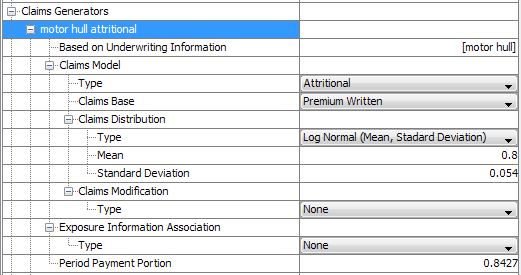
\includegraphics[scale=0.6]{images/ClaimsGenerator.png}
	\caption{Claims Generator: Motor Hull Attritional}
	\label{fig:ClaimsGenerator}
\end{figure}

\subsection{Underwriting Information}
\label{subsec:UWInfo} 
 
As your first selection, you have to decide on which \term{Underwriting Information} your claims generator will be based\footnote{It is also possible to run a simulation for claims generators and reinsurance only. However, if you want to calibrate the claims generator not only by \term{absolute} values but rather by \term{premium} or similar, this information must be provided here.}: As a starting point, you will usually select one underwriting segment per claims generator and vice versa. Given the situation, where you have data available for two similar underwriting segments -- such as `motor tpl own business' and `motor tpl co-insured business', both with the same characteristics but internally treated separately for regulatory reasons -- you can use the same claims generator for both of them. This will reduce the maintenance of your model as there will be less parameters to update and less time needed for the simulation procedure.\footnote{However, this simplification will add a maybe unwanted dependency between the two underwriting segments. Better creaty a duplicate of the first claims generator by right-clicking on the existing claims generator.} Essentially, any Underwriting Segement as setup within the given parameterization (\cf~Section~\ref{sec:underwritingsegments}) and an `additive' combination thereof is a valid selection for basing a claims generator on it. 
 
Having a look at a simulation from the other end, you will find the following components being usually requesters of underwriting information:


\begin{itemize}
	\item claims generators, as their calibration may be based on sum insured, premium, or number of policies,
	\item frequency generators -- as an element of claims generators -- in case being calibrated based on number of policies,
	\item allocation of sum insured to claims,
	\item proportional reinsurance contracts where they need gross underwriting information in order to calculate the ceded underwriting information, or
	\item working/cat excess of loss and stop loss reinsurance contracts where as the ceded premium may be specified as GNPI, rate on line or number of policies.

\end{itemize}
 
\subsection{Claims Model}
\label{sec:ClaimsModel}
\label{subsec:ClaimsModel}

Depending on the application, a Claims Model \term{Type} from Table~\ref{tab:ClaimsModelType} can be selected. The Claims Model Type defines the form of the claims model; the names and structure of subordinate parameters depend on it. The default value \term{None} provides an empty Claims Generator, producing no claims. \\ The intent of the \term{none} type is to easily toggle a claims generator on or off, e.g.~in case you want to use it in the first period but not in the second period of a multi-period model. 

\begin{table}[htbp]
	\centering
		\begin{tabular}{lll}
			\textbf{Claims Model Type} & (Additional) \textbf{Input Fields} & \textbf{Example} \\
			None & \textit{Disabled} & \textit{No Claims produced} \\
			Attritional & Claims Base & Premium Written \\
				& Claims Distribution & Poisson$(\lambda)$ \\
				& Claims Modification & Truncated (min, max), Shift\\
			Attritional with Date & \textit{with a random incurred Date} & Uniform$(0.4,0.8)$ \\
			Frequency Average Attritional & Frequency Base & Number of Policies \\
				& Frequency Distribution & Binomial$(n, p)$ \\
				& Frequency Modification & Censored (min, max) \\
			Frequency Severity & \textit{no additional fields} \\
			Frequency Severity with Date & Occurence Distribution & Normal$(\mu, \sigma)$\\
				& Produce Claim & Single Claims \\
			Severity of Event Generator & \textit{no additional fields} \\
		\end{tabular}
	\caption{Claims Model Types}
	\label{tab:ClaimsModelType}
\end{table}

\subsubsection*{None}

This selection is useful for quickly de-activating an already defined claims generator e.g.~for setting up a multi period model where a specific claims generator is active only during a limited number of periods.

\subsubsection*{Attritional}

Modelling `attritional' claims is started by selection of the claims base as measure of calibration of the simulated claims. 
This calibration directly refers to the underlying underwriting information stored in \term{Underwriting Segments}. 
Let us choose to scale our claims by \term{sum insured} where the non-scaled claims distribution is given by a lognormal distribution LogNormal$(0.8;0.054)$. 
The selection above will result in non-scaled claims with mean $0.8$ and standard deviation $0.054$.

The scaled claims, as defined by multiplying a given constant -- such as the sum insured in this example -- with the non-scaled claims, are again lognormal distributed with parameters LogNormal$(0.8$ $*$ Sum~Insured; $0.054$ $*$ Sum~Insured).

Assuming we will have to update our model some months later, as a first step, we might want to update
just the sum insured amount, automatically getting a model based on both the updated sum insured amounts,
to reflect a growing portfolio, as well as the parameters selected during the last exercise.
Assuming again that we now want to update not only the sum insured, but also the mean of the distribution,
which we found to be too low by 3\%, selecting \term{Shift} as \term{Claims Modification} will allow us to
shift the claims manually based on our calibration exercise. 

The parameter used for shifting will modify
the distribution before being applied to the scaling measure; \ie, for a given shifting parameter $a$, $a=0$
will result in no shift, while $a \neq 0$ shifts the generated claims either positively or negatively.
In descriptive words: claims generator$_{shift_{a}}$ = $($claims distribution $+$ $a)$ $*$ scaling measure: Assuming a sum insured of EUR 1bn, the claims distributed as specified above and now shifted by a factor of
$a$ = $0.8*0.03$ = $0.024$ would inflate the simulated claims $C$: $C$ = LogNormal($0.8 + 0.024;0.054)$ $*$ EUR 1bn. \\
An overview and explanation of all possible selections is given in the table on page~\pageref{tab:ClaimsModelTypeDetail}.

\subsubsection*{Attritional with Date}\label{sec:AttritionalClaimDate}

Whereas attritional claims are per default modelled as one aggregated (\ie~grouped) claim occuring in the middle of the period (e.g.~30 June of a standardized year), the user has the possibility to select a statistical method for allocation of a date within the time period to the simulated claim. In many situations it is important to know, when a claim occurred, namely for reinsurance contracts incepting during the period and therefore not covering the whole period as being modelled. For seasonal business such as a hail cover in Europe it might make sense to select Uniform$(0.4;0.8)$ resulting in one attritional claim occuring -- based on the selected claims distribution -- sometime between May and October. If you setup a one-year reinsurance contract with inception date 1.~January, all claims occuring during this period will be covered by the reinsurance contract. But if you setup a reinsurance contract with inception date on 1.~October, the reinsurance will not cover the hail claims in each and every iteration.

\subsubsection*{Frequency Average Attritional}

This selection is used for modelling claims with more details than `just attritional' and less than a classical frequency-severity model as it still aggregates to claims to being one. While the former ('attritional') results in one attritional claim per time period, and the latter ('frequency severity') in several claims with different severities, the selection here is used for modelling one  attritional claim as specified above but by using a different kind of parameterization. The user might select a constant distribution of $5$ resulting in one attritional claim being parameterized by the number (frequency) of five claims and the severity as specified.

\subsubsection*{Frequency Severity}

A very flexible claims generator is made available through this option: In addition to specific modelling of both, frequency and severity of the claims, the user has the option to group the simulated claims to one event selecting \term{Produce Claim} as \term{Aggregate Event Claims}; this has an impact on some reinsurance programs.

\subsubsection*{Frequency Severity with Date}

In addition to the already explained claims model \term{Frequency Severity} the hereby explained model allows the modelling of assumptions around the occurence of the claims. As default, a uniform$(0;1)$ distribution is applied, resulting in equally distributed claims over the complete time period. Alternatively, for example, Piecewise Linear$((0;0.25;0.5;1);(0;0.33;0.66;1))$ would result in an occurence pattern with no occurences from January to March, $33/100$ of claims occuring between April and June, another $33/100$ between July and December and the remaining $34/100$ on the latest day of the (standardized) year. Again, this is important to know namely for reinsurance contracts incepting during the period and therefore not covering the whole period as being modelled.

\subsubsection*{Severity of Event Generator}
\label{sec:ExternalSeverity}

Severity of event generator is selected in case you want to first simulate severities by use of the \term{Event Generator} (\cf~the section on \term{Event Generators} on page~\pageref{sec:eventgenerator} for more details) and afterwards apply them to -- usually -- several underwriting segments: By using this approch, the \term{Event Generator} (\cf~Section~\ref{sec:eventgenerator}) will firstly draw one or several event as specified in your parameterization whereof a percentile is drawn. This percentile then gets applied to the \term{Claims Distribution} here.

\begin{table}[p]
    \centering
        \begin{tabular}{|l|p{11 cm}|}
          \multicolumn{2}{c}{This is a summary of names and entries for comboboxes as related to claims generators.} \\
            \hline
            \textbf{Name}, Combobox&\textbf{Description} \\
            \hline
            \textbf{Type} & \textbf{Selection of Claims Model Type}\\
            None & No claims are generated.\\
            Attritional & One attritional claim is generated occuring in the middle of the time period: $1$ claim occuring on 30 June of a standardized year.\\
            Attritional With Date & One attritional claim is generated occuring during the time period based on a specified distribution:  $1$ claim per period with randomly distributed occurrence date (attached to the claim for further use!).\\
            Frequency Average Attritional & One attritional claim as per the specified parameters is simulated.\\
            Frequency Severity & Distributions for both, frequency and severity, are specified. \\
            Frequency Severity with Date & Frequency and Severity model including distribution of the occurrence. Dates are attached to the claim for further use. \\
            Severity of Event Generator & Please see the sections on \term{severity of event generator} (page~\pageref{sec:ExternalSeverity}) and on \term{Event Generators} (page~\pageref{sec:eventgenerator}). \\
            \hline
            \textbf{Frequency Base} & \textbf{Specification of multiple to the mean of the specified claims frequency}\\
            Absolute & The mean of the distribution is pre-determined as absolute value;\\
            Number of Policies & or by the number of policies.\\
            \hline
            \textbf{Frequency Distribution} & \textbf{Please refer to the \href{http://www.iro.umontreal.ca/~simardr/ssj/indexe.html}{SSJ Library}} \\
            \hline
            \textbf{Frequency Modification}& \textbf{Applying a modification to the claims generator \textit{before} multiplying with the Frequency Base}\\
            None & No modification to the selected frequency distribution. \\
            Truncated & Cutting the distribution at a specified minimum and maximum value respectively. No observations outside the given range are observed. Applying a deductible is an illustrative example for truncation at the lower end of the distribution: lower claims are not registered. \\
            Truncated, Shift & Combination of both methods by first truncating and afterwards shifting the distribution. \\
            Censored &  Censoring the distribution at a specified minimum and maximum value respectively. Any observation outside the given range is `rounded' to lie within the range. Applying a maximum sum insured is an illustrative example for censoring at the higher end of the distribution: higher claims are cut to the maximum sum insured.
            \\
            Censored, Shift & Combination of both methods by first censoring and afterwards shifting the distribution. \\
            Shift & Additive shifting of the mean of the distribution by the parameter.\\
            \hline
            \textbf{Claims Base} & \textbf{Specification of multiple to the mean of the specified claims severity}\\
            Absolute & The mean of the distribution is pre-determined as absolute value;\\
            Premium Written & or by written premium,\\
            Number of Policies & by number of policies, or\\
            Sum Insured & by sum insured.\\
            \hline
            \textbf{Claims Distribution}& \textbf{Please refer to the \href{http://www.iro.umontreal.ca/~simardr/ssj/indexe.html}{SSJ Library}}\\ & Discrete Empirical (cumulative) allows to load external information such as RMS-tables. \\
            \hline
            \textbf{Claims Modification}& \textbf{\cf~above \textit{Frequency Modification}}\\
            \hline
            \end{tabular}
    \caption{Claims Model: Summary and Explanations of Comboboxes}
    \label{tab:ClaimsModelTypeDetail}
\end{table}

\subsection{Exposure Information Associaton} 
\label{subsec:Exposure Information Associaton}
As in some cases the size of a claim is not sufficient for the following depending calculations, exposure information, like the sum insured (SI) and the probable maximum loss (PML) can be attached to the claim. Especially the surplus reinsurance cover requires to know pairs of exposure and claim size to calculate the coverage.\footnote{Surplus reinsurance is a more advanced and more complicated form of proportional reinsurance where the portion covered by the reinsurer depends on the sum insured (or other quantities) specified for the underlying insured risks. The portion of the claim ceded to the
reinsurer is given by the ratio of the risk ceded divided by the total risk.} Except \term{None} there are two exposure information association mechanisms available: \term{Risk to Band} and \term{Sum Insured Generator}; all of them explained further below. 

In principle, there are many different ways of allocating claims to risk bands. \RiskAnalytics{} offers two different approaches, one of which is applied
to aggregate losses and the other to single losses. In both approaches, the allocation uses a target allocation that specifies for each risk class the percentage of claims that should be associated with the
given risk class. In the case of aggregate claims, the target allocation can always be easily met since aggregate claims can always be split up. 

\subsubsection*{None}
In case no exposure association to the claims is needed, this selection is appropriate. If, on the other hand, the exposure association is needed but not specified here, the portion of ceded risk is set to zero even if an instrument such as surplus reinsurance is specified further below in the parameterization. 

\subsubsection*{Risk to Band}
\label{subsubsec:riskToBand}

In case of single claims, the following modified procedure is applied: For an initial guess, the incoming (individual) losses are allocated to the risk
classes by just referring to the claim size, \ie~the claim must fit in between the lower and the upper limit of the risk band. Based on the selection such as \term{Premium}, an algorithm re-alocates the single claims to higher risk bands where needed in order to allow a best-fit to the weight per band as set by \term{Premium} (in this example).

\subsubsection*{Sum Insured Generator}
The sum insured generator produces the required exposure information using the claim and the maximum sum insured. The claim ($X_i$) is used as generated from the claims generator, the maximum sum insured or PML is taken from the appropriate underwriting information. The sum insured is calculated using the following formula $SI_i= a (PML-X_i)+X_i$. The random distribution $a$, usually $a\in [0,1]$, is configurable by the parameters of the sum insured generator. 

Furher details on surplus reinsurance are explained in Section~\ref{subsec:Surplus} on page~\pageref{subsec:Surplus}. 

\subsection{Period Payment Portion} 

The parameter period payment portion $p$ is part of the reserve model (\cf~Section~\ref{sec:ReserveGenerators}). The share $p\in[0,1]$ is the part of a generated claim which is paid during the current period. The share $1-p$ is shown as reserved at the end of the period.
 
\section{Reserve Generators}
\label{sec:ReserveGenerators}

The reserve generators provide an additional option to model random effects of IBNyR/IBNeR. 
As a volume parameter the initial reserve volume can be put in. The reserve generator allows for the \todo{types listed below}{tbd}.

\begin{figure}[htb]
	\centering
		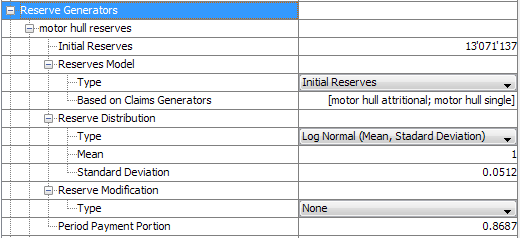
\includegraphics[scale=0.6]{images/ReserveGenerator.png}
	\caption{Reserve Generator}
	\label{fig:ReserveGenerator}
\end{figure}

More details are explained in the specific chapter on page~\pageref{chap:nl-reserves}\,\ff



\section{Dependencies} 
\label{sec:ClaimDependencies}

This is a short overview only. For more details, please refer to chapter \ref{chap:dependencies} on pages \pageref{chap:dependencies}ff.

Given a portfolio with two underwriting segments, for instance \term{motor hull private} and \term{motor hull commercial}, dependencies in-between these two underwriting segments will occur: By selecting a dependency for two or more underwriting segments, all \term{attritional} and/or \term{attritional with date} claims will be modelled with the specified dependency.

\begin{figure}[htb]
	\centering
		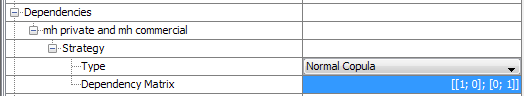
\includegraphics[scale=0.6]{images/Dependency.png}
	\caption{Dependencies}
	\label{fig:Dependencies}
\end{figure}

\begin{figure}[htb]
	\centering
		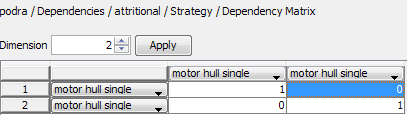
\includegraphics[scale=0.6]{images/dependency_matrix.png}
	\caption{Dependency Matrix}
	\label{fig:Dependencies}
\end{figure}

Whilst such dependecies are usually not linear, 
they are modelled by use of copulae belonging to these families:
\begin{itemize}\tightitemize{0pt}
	\item  \term{Normal} (Gaussian), specified by a dependency matrix
	\item  \term{Frechet upper bound}, applied to a target, \ie~a claims generator
	\item  \term{No Correlation}, \ie~independent targets
	\item  \term{T-Copula}, specified by the degrees of freedom and a dependency matrix
	\item  \term{Gumbel}, specified by parameters Lambda, the dimension and the targets
\end{itemize} 

Whilst further details on how to use dependencies in \RA are given in the respective chapter on page~\pageref{chap:dependencies}\,\ff{}.Details on the implementation of these copulae can be found here \href{www.link.me$\backslash$please}{www.link.me$\backslash$please}; details on how to calibrate the dependency structure given a specific portfolio are usually provided together with spezialized calibration software. \PO{} \RA{} releases come with parametrizations that furnish examples of companies having dependencies between selected underwriting segments.

\section{Event Generators}
\label{sec:eventgenerator}

\todo{Event Generator vs Event Correlation in MCM}{todo}
An insurance contract always specifies the covered risk: Some reinsurance contracts cover the complete balance sheet of a company (such as Stop Loss), others only cover one specific building or vehicle (such as facultative reinsurance cover for the construction of a tunnel). XL treaties usually either are specified as \term{per risk} or \term{per event}. In the latter case, an often high number of -- relatively -- small claims lead to a large loss for the insurance company; however, none of these small claims would be covered by reinsurance separately. So we would have to select a claims generator with the option \term{Produce Claims: Aggregated Event}.

\begin{figure}[htb]
	\centering
		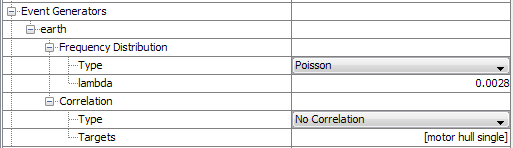
\includegraphics[scale=0.6]{images/EventGenerator.png}
	\caption{Event Generator}
	\label{fig:EventGenerator}
\end{figure}

If you select an \term{Event Generator} it will simulate the severity of an event by determining the percentile -- as number between 0 and 100. If for example, the percentile of $84\%$ is drawn, this percentile is fed to the claims generators where the option \term{severity of event generator} is selected. Depending on the loss distribution for each underwriting segment the loss amount will be calculated depending on the specified percentile.\todo{}{This section needs rewording and more explanation. the first paragraph is really misleading!}

